\label{5_resultados}

\section{Parâmetros analisados}

Como um AG trabalha com tentativa-e-erro, não há uma geração exata para a qual pode ser prevista uma determinada solução (ou proximidade à solução). Para se analisar a evolução dos indivíduos ao longo das gerações, este trabalho focou em analisar os seguintes parâmetros:

\begin{itemize}
	\item Valor mínimo de fitness em um indivíduo;
	\item Valor máximo de fitness em um indivíduo;
	\item Valor médio de fitness entre todos os indivíduos;
	\item Desvio padrão dos valores de fitness.
\end{itemize}

O desvio padrão utilizado aqui foi o amostral, dado por:

\begin{equation}
	\sigma = \sqrt{\frac{1}{N-1} \sum_{i=1}^N (x_i - \overline{x})^2}
\end{equation}

Os gráficos criados tiveram como base uma única simulação do AG para o problema e parâmetros de entrada escolhidos. Não é possível ter expectativas de valores ou gerações, uma vez que o AG trabalha com tentativa-e-erro, então criá-las ou assumi-las seria difícil de quantizar.

Como já foi comentado antes, se não for mencionado o contrário (mesmo para o caso adaptativo), utilizou-se 0.9 para $p_c$ e 0.01 para $p_m$. Todas as execuções utilizaram 100 indivíduos, 200 gerações e elitismo do melhor indivíduo. Se um problema convergiu completamente para a melhor solução antes das 200 gerações completarem, os gráficos foram reduzidos para melhor visualização, uma vez que os pontos extras não trariam novas informações para nós.

As simulações feitas com uso do AGA foram utilizadas para comparação com a implementação estática do AG. Além disso, foi avaliado o comportamento adaptativo de $p_m$ ao longo das gerações.

\section{OneMax Booleano}

\subsection{Caso Estático}

Este problema foi considerado simples de ser resolvido por um AG, uma vez que poucas mutações em um gene já permitem que ele ficasse igual a 1. As figuras \ref{fig:onemax_boolean} e \ref{fig:onemax_boolean_std} demonstram exatamente isso, com convergência completa dos indivíduos para a solução ótima após 93 gerações, sendo que a própria solução ótima foi encontrada com a melhor solução aparecendo após 78 gerações.

\begin{figure}[ht!]
    \centering 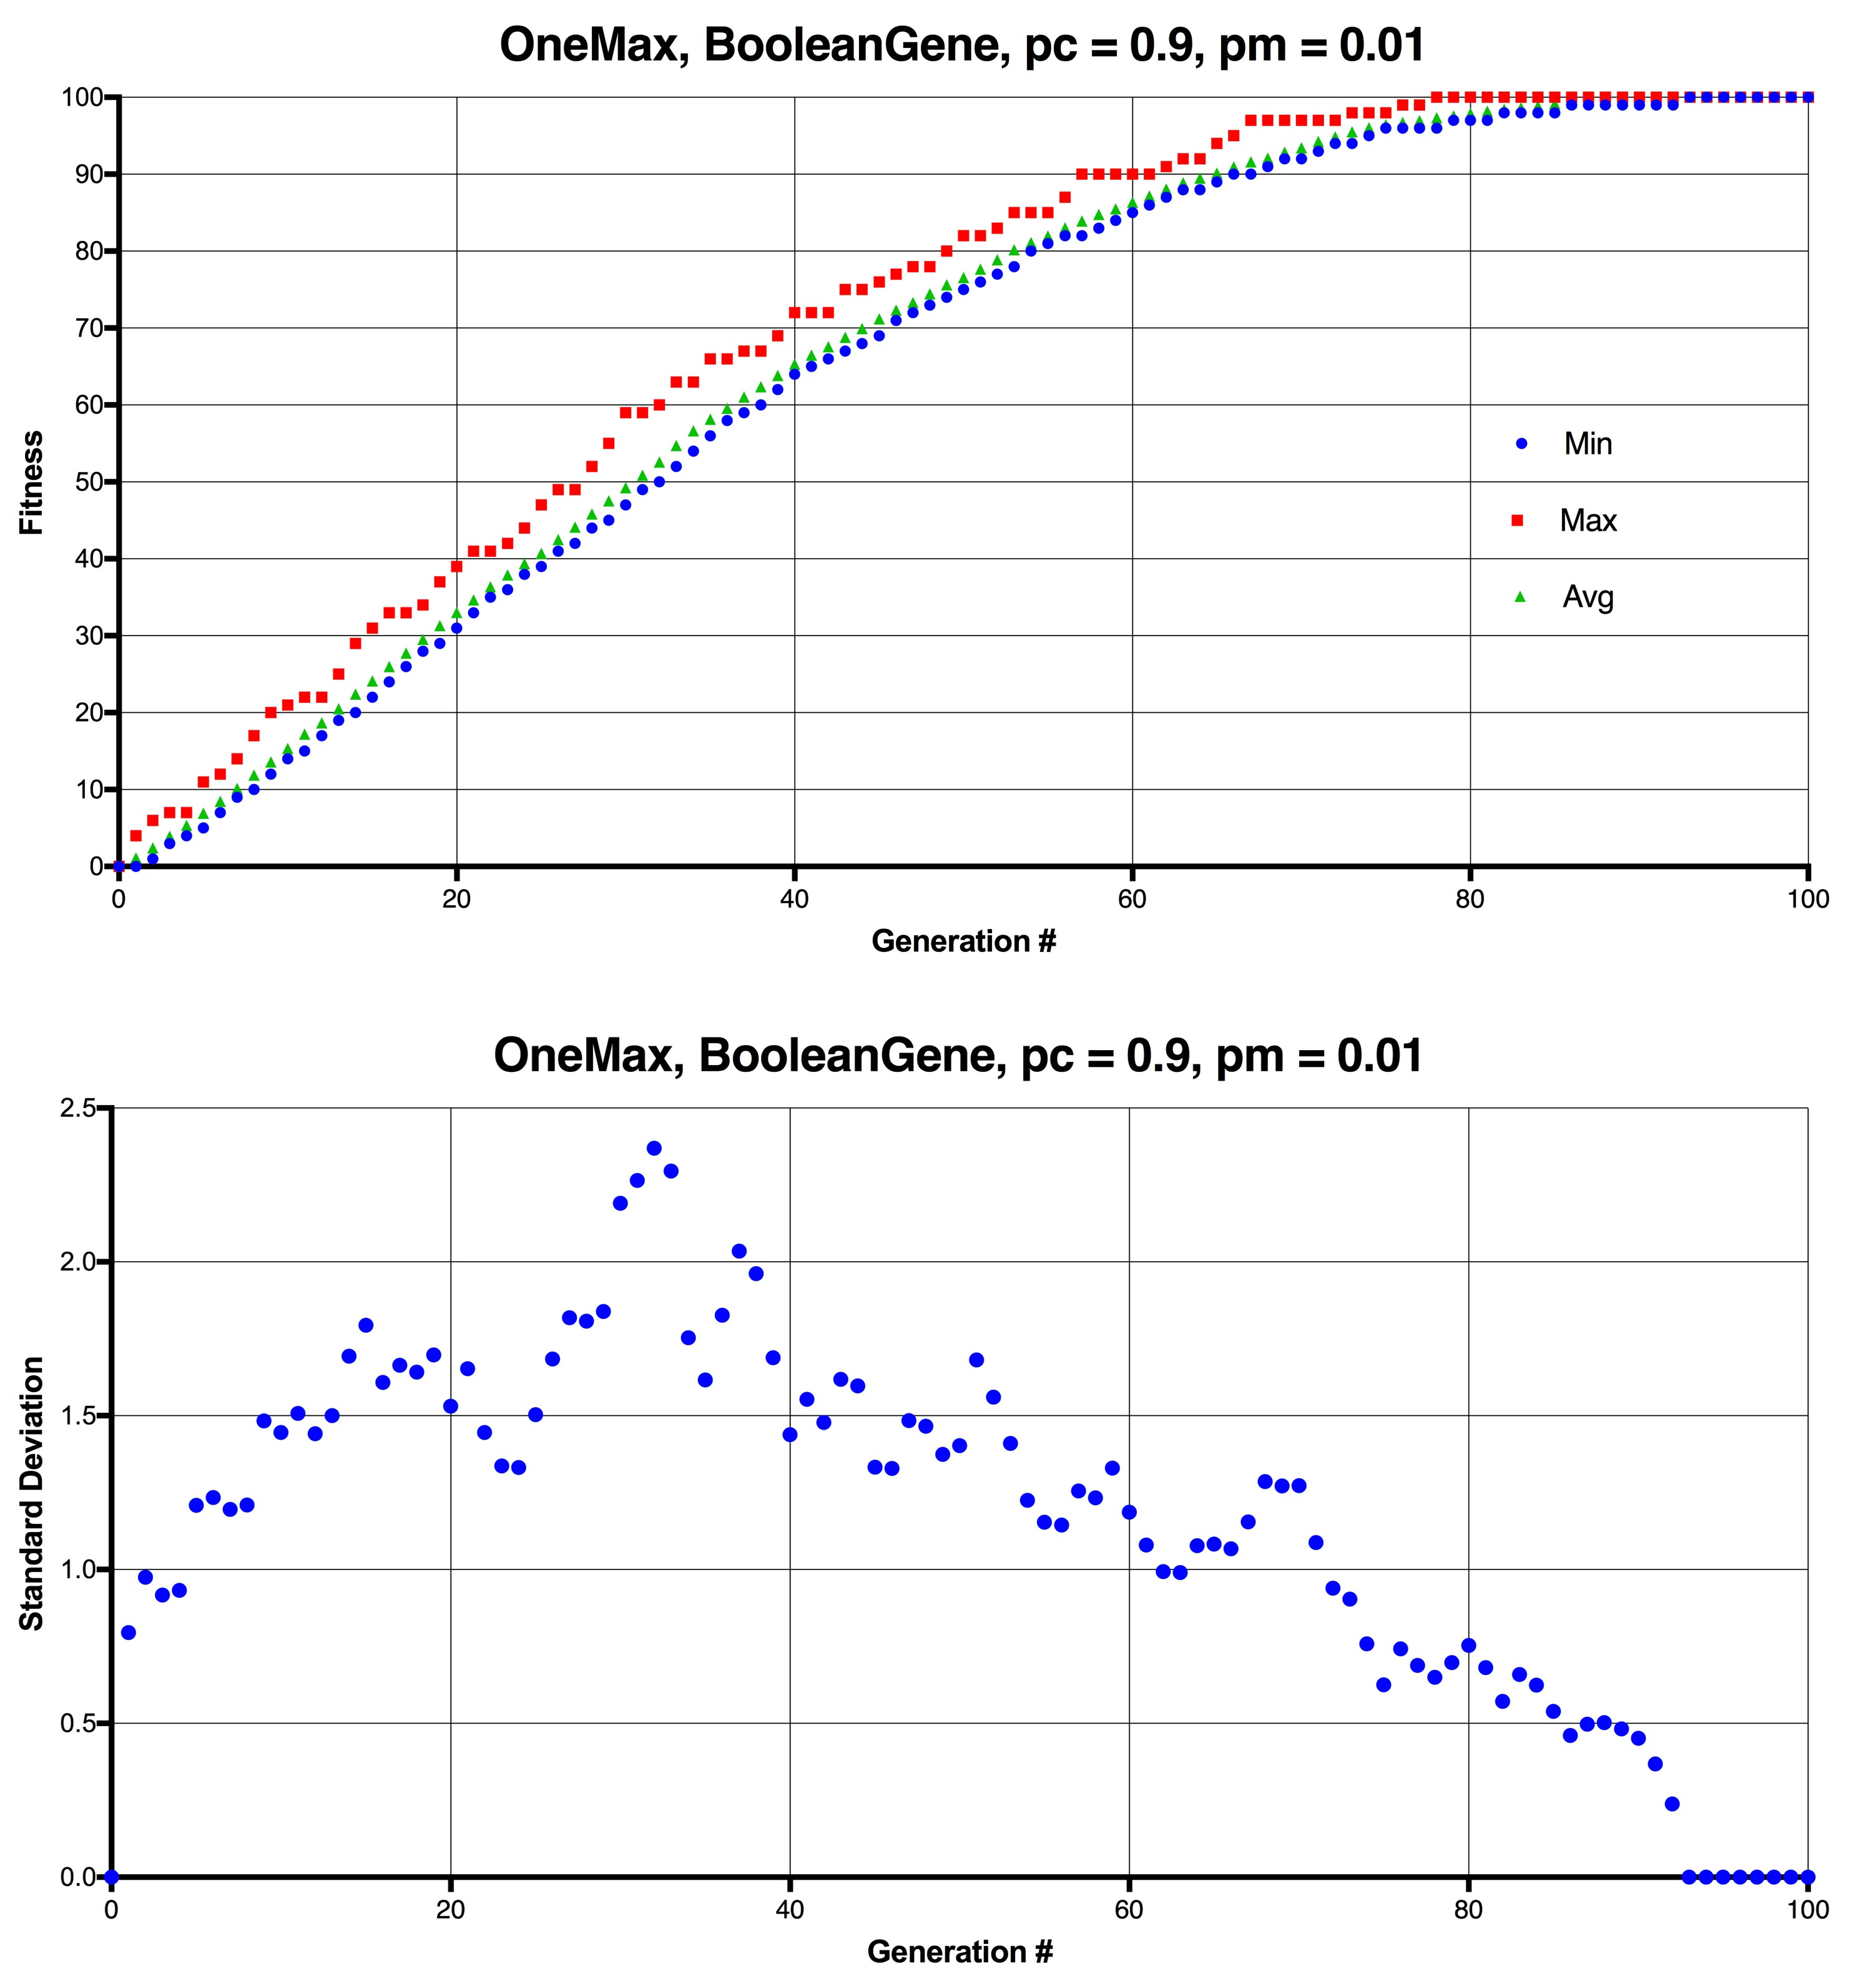
\includegraphics[width=1.0\textwidth]{onemax_boolean.jpg}
    \caption{Evolução do fitness para o problema do OneMax Booleano mostrando mínimo, máximo e valor médio ($p_c=0.9$, $p_m=0.01$). Foram necessárias 78 gerações para que a solução ótima aparecesse, e 93 gerações para que todos os indivíduos convergissem para ela.}
    \label{fig:onemax_boolean}
\end{figure}

\begin{figure}[ht!]
    \centering 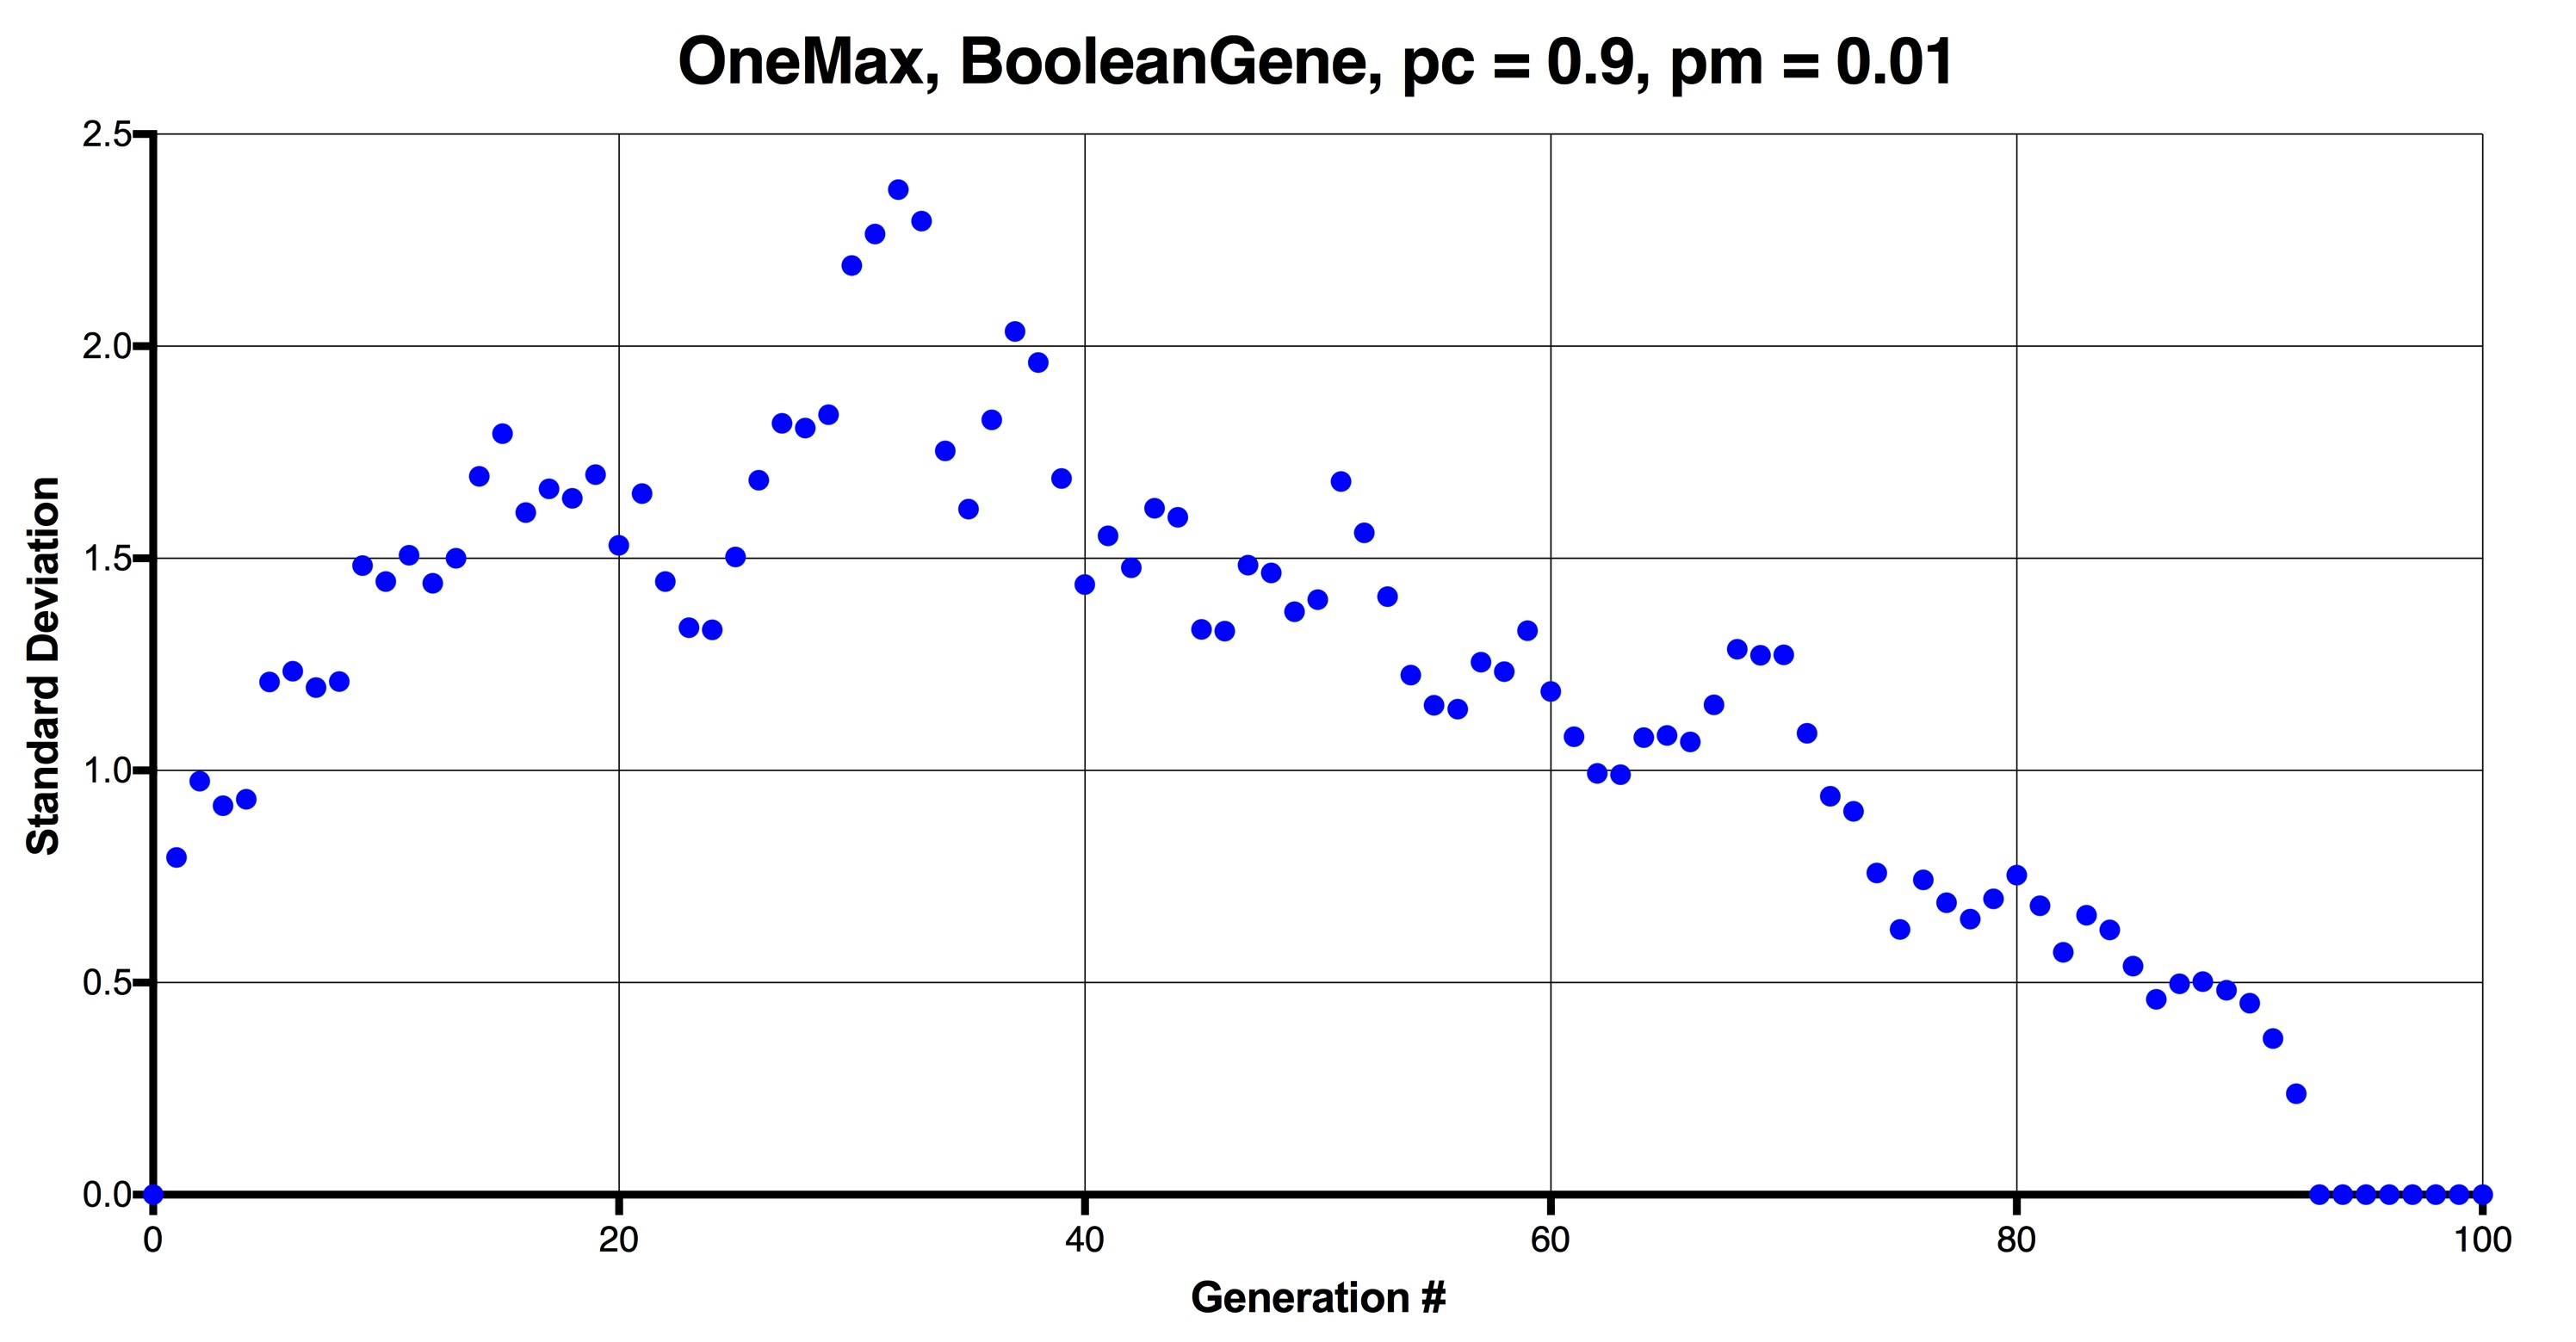
\includegraphics[width=1.0\textwidth]{onemax_boolean_std.jpg}
    \caption{Desvio padrão ao longo das gerações para o problema do OneMax Booleano ($p_c=0.9$, $p_m=0.01$).}
    \label{fig:onemax_boolean_std}
\end{figure}

O comportamento estático para os valores padronizados de $p_c$ e $p_m$ mostrou um crescimento aproximadamente linear dos valores de fitness, tanto para o pior quanto para o melhor indivíduo. Isso demonstra que tais valores demonstram um crescimento equilibrado da população, e a mutação existente é suficiente para evoluir os indivíduos.

\subsection{Caso Adaptativo}

Com o AGA ativado, ficou bem mais complicado para o OneMax atingir a solução ótima. Como mostrado na figura \ref{fig:onemax_boolean_adaptive}, foram necessárias 113 gerações para que o melhor indivíduo atingisse a solução ótima, e a média dos valores de fitness oscilou entre 93 e 95 para as últimas gerações. Em termos de desvio padrão, como mostrado na figura \ref{fig:onemax_boolean_adaptive_std}, o valor nunca passou de 2.0 (de um máximo de 100), o que nos diz que a população não se dispersou completamente pelo efeito adaptativo.

\begin{figure}[ht!]
    \centering 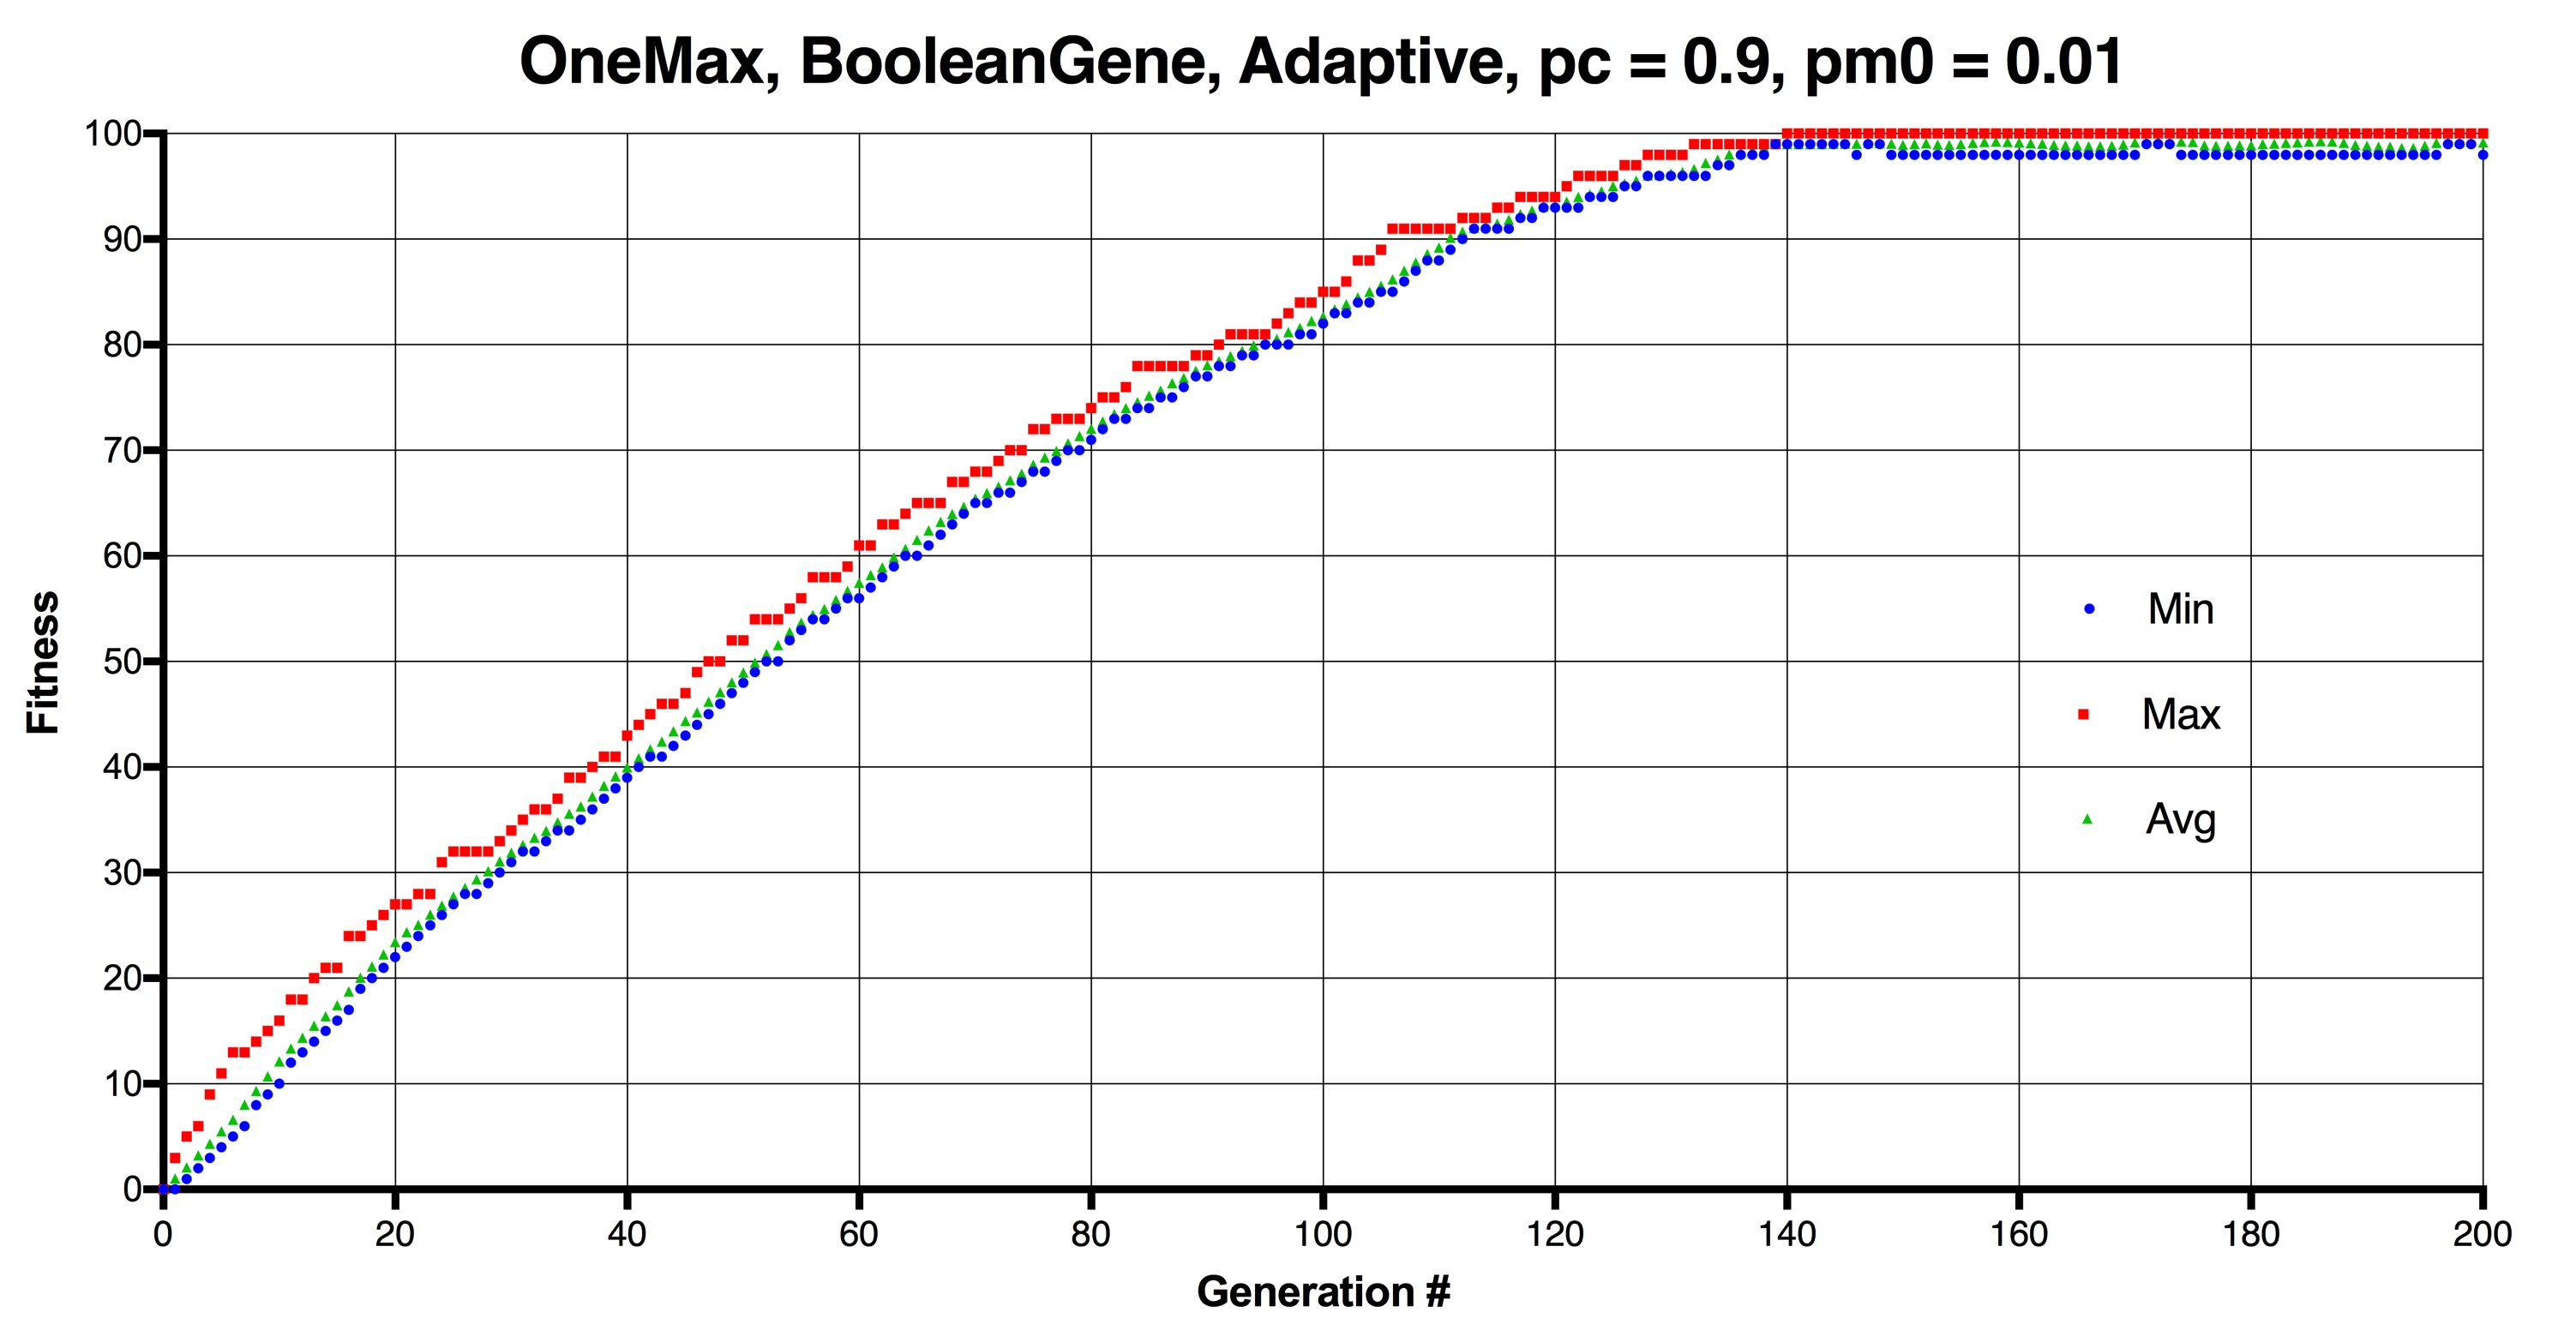
\includegraphics[width=1.0\textwidth]{onemax_boolean_adaptive.jpg}
    \caption{Evolução do fitness para o problema do OneMax Booleano Adaptativo mostrando mínimo, máximo e valor médio ($p_c=0.9$, $p_{m0}=0.01$). Foram necessárias 113 gerações para que um indivíduo encontrasse a solução ótima.}
    \label{fig:onemax_boolean_adaptive}
\end{figure}

\begin{figure}[ht!]
    \centering 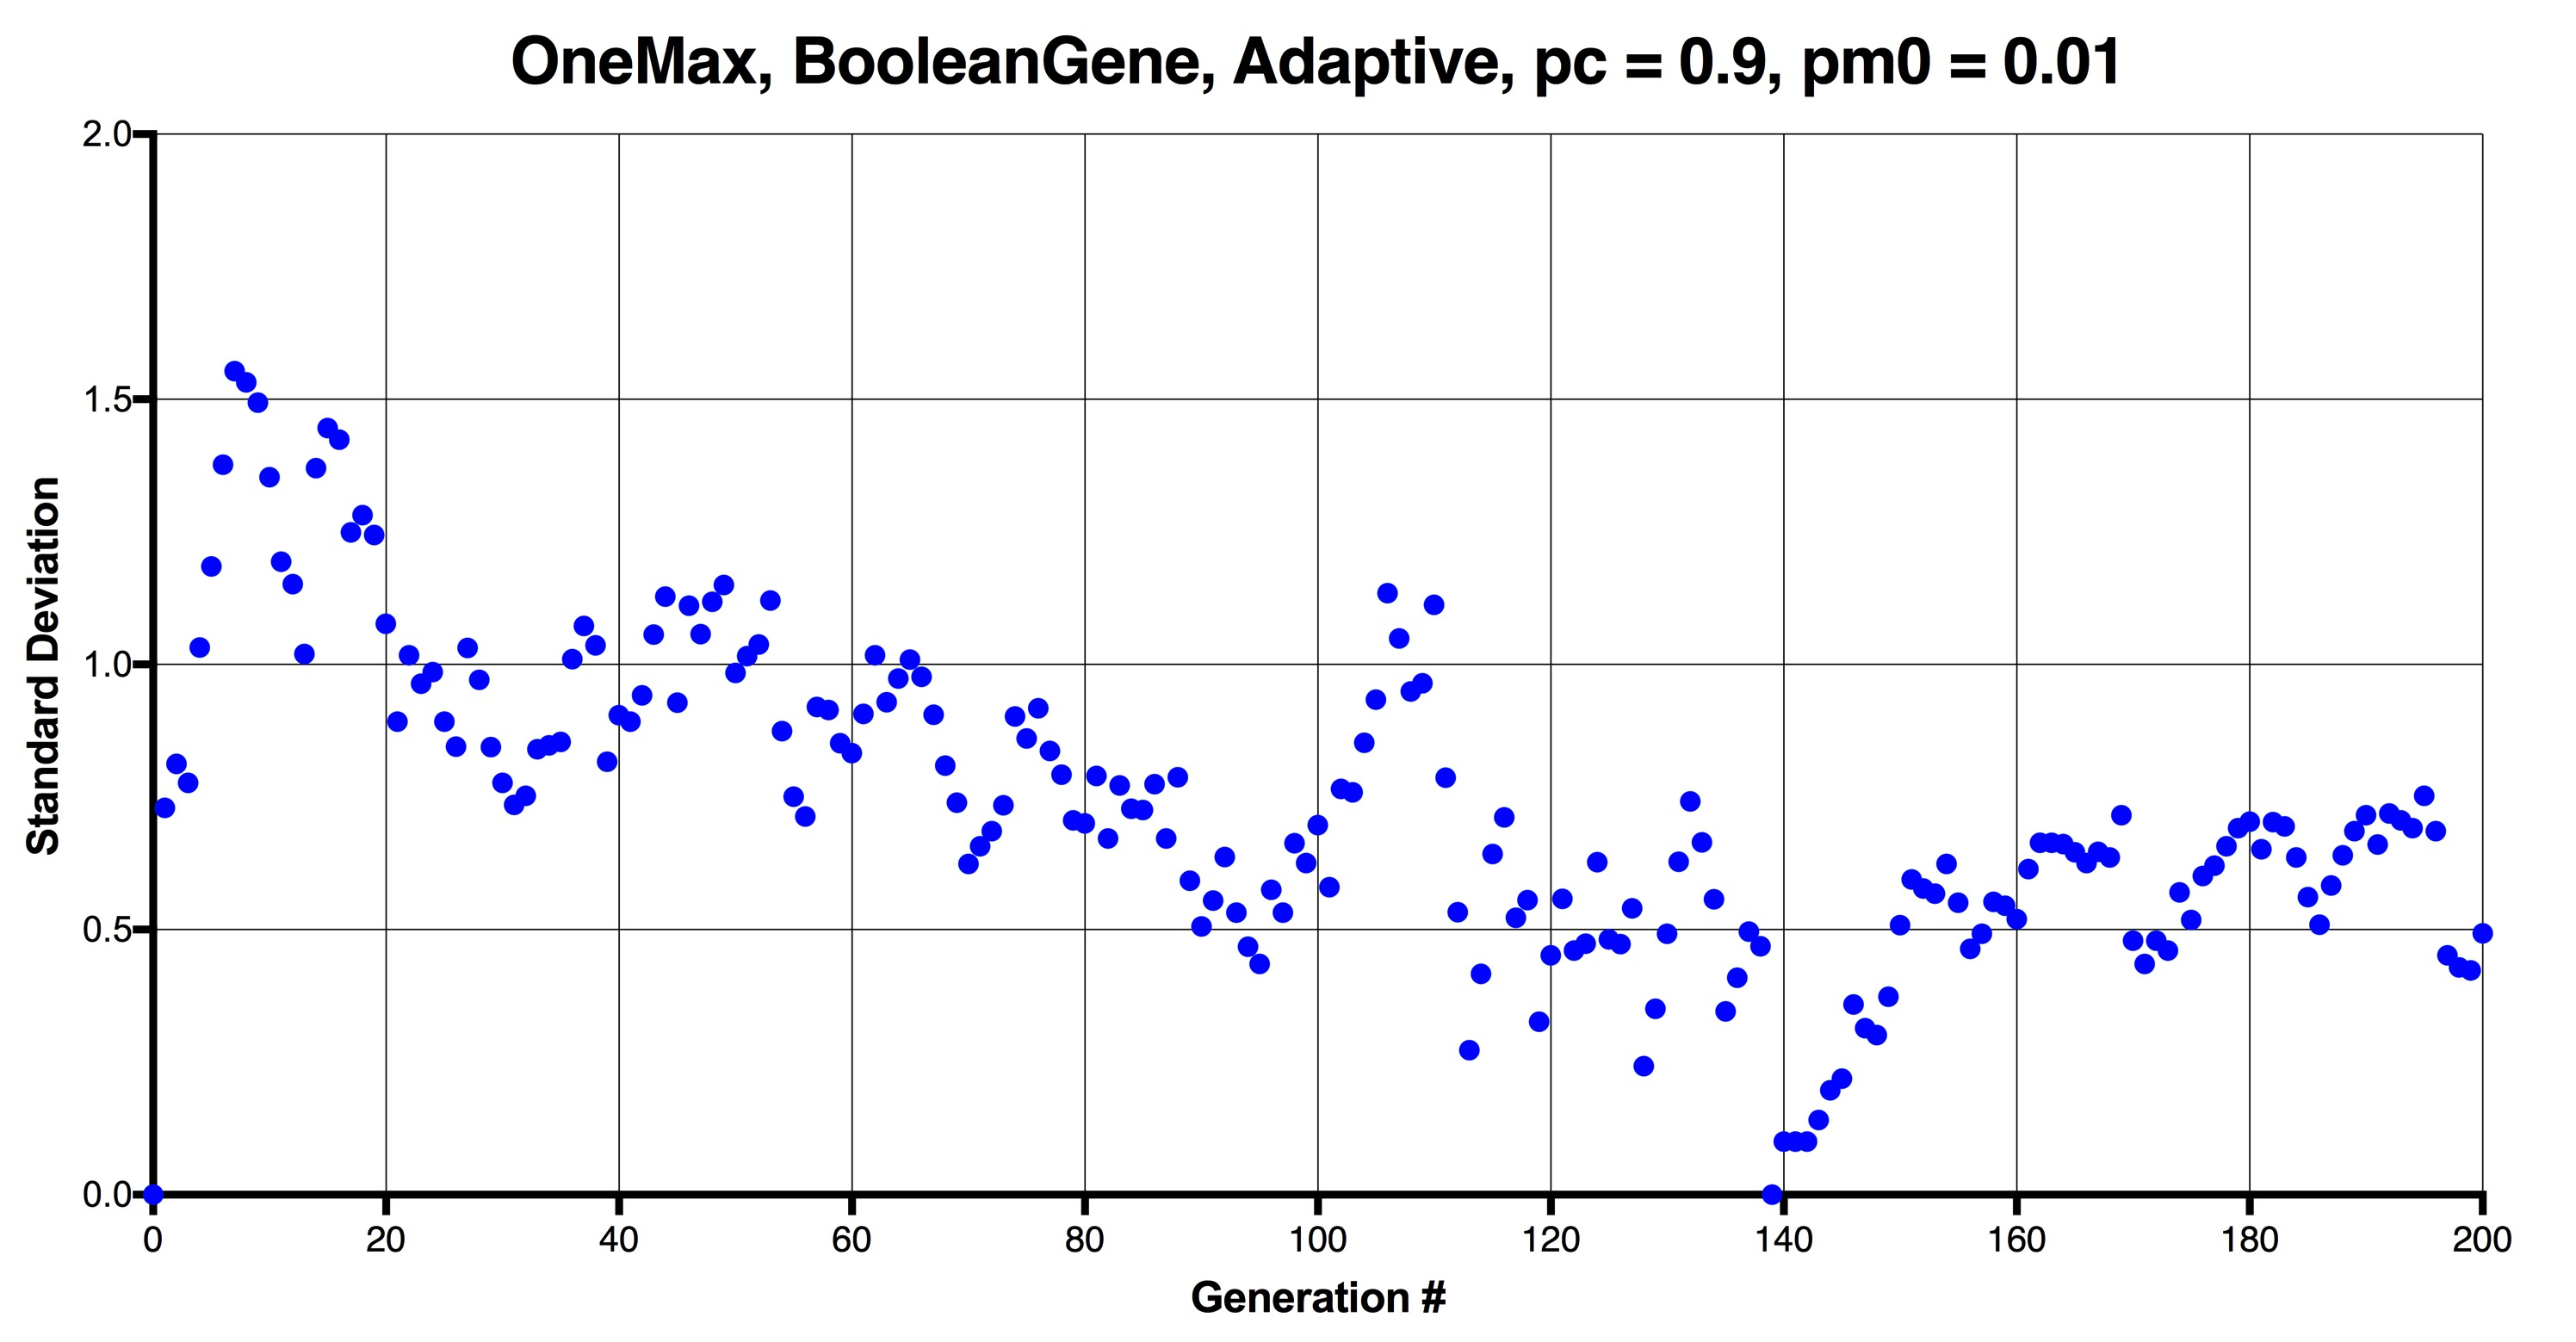
\includegraphics[width=1.0\textwidth]{onemax_boolean_adaptive_std.jpg}
    \caption{Desvio padrão ao longo das gerações para o problema do OneMax Booleano Adaptativo ($p_c=0.9$, $p_{m0}=0.01$).}
    \label{fig:onemax_boolean_adaptive_std}
\end{figure}

Um efeito interessante pode ser visto na figura \ref{fig:onemax_boolean_adaptive_pm}, com relação à evolução de $p_m$ e $p_{m0}$. É possível ver que as primeiras gerações ainda eram muito dispersas, o que fez com que $p_m$ começasse a cair. No entanto, como mencionado antes, um valor baixo de $p_m$ se mostrou mais do que suficiente para que a população do caso estático fosse capaz de encontrar a solução ótima.

\begin{figure}[ht!]
    \centering 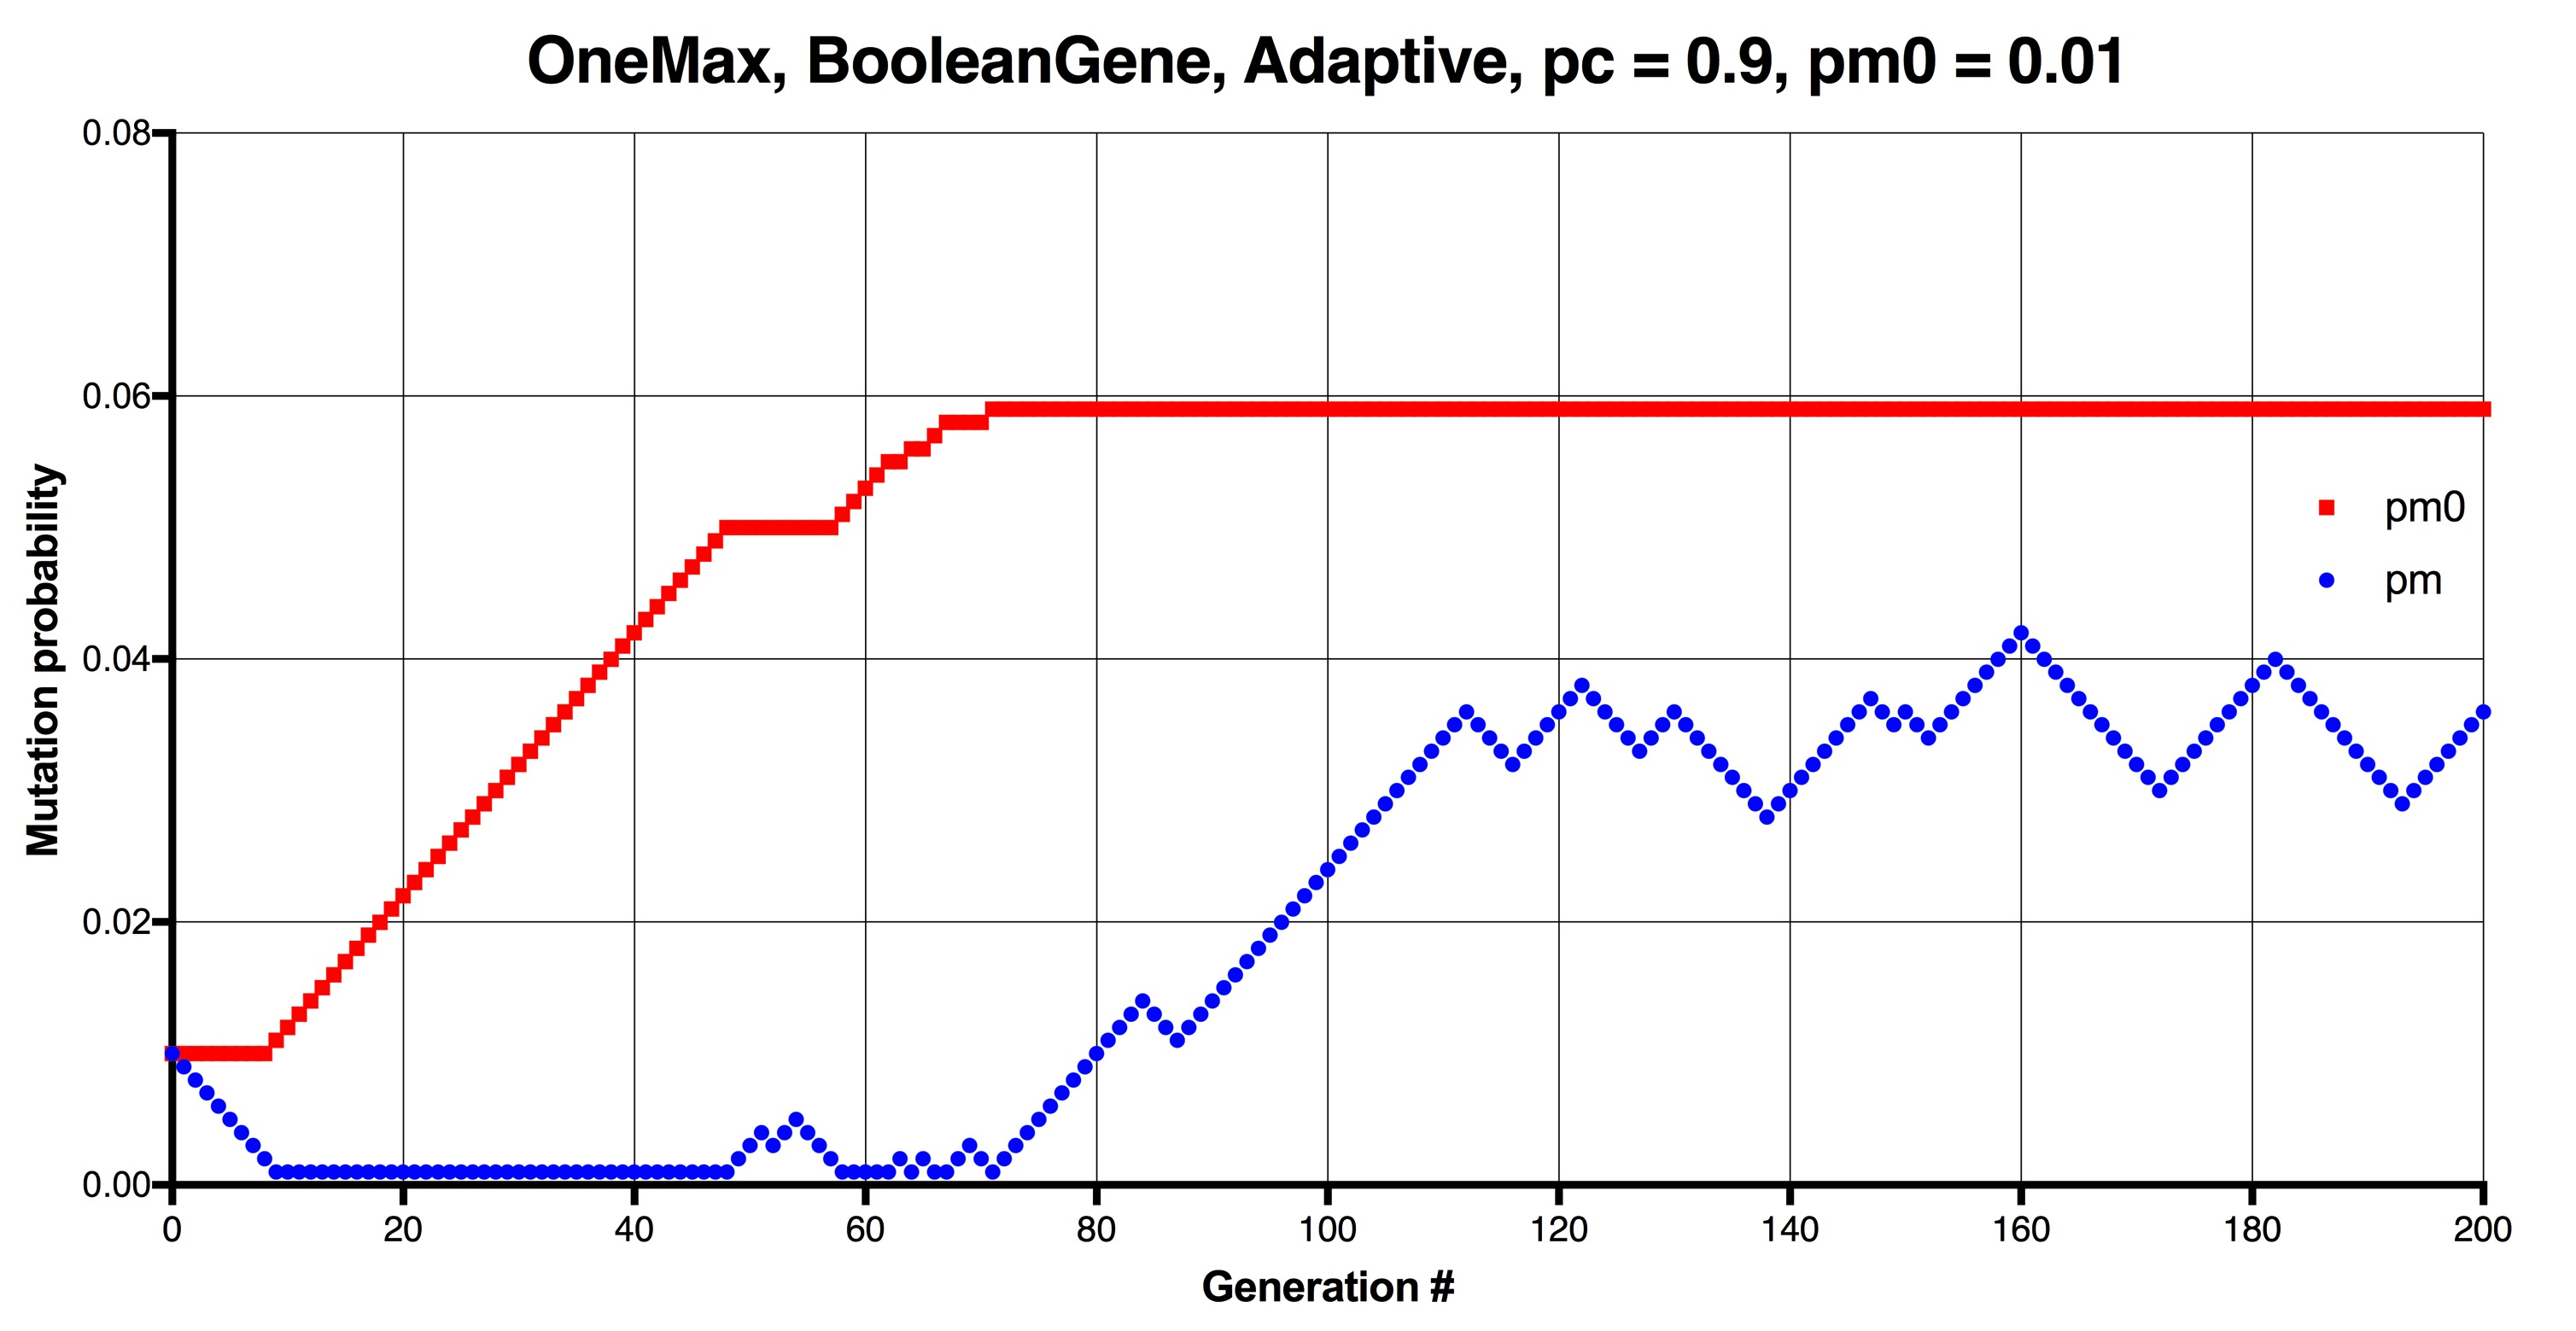
\includegraphics[width=1.0\textwidth]{onemax_boolean_adaptive_pm.jpg}
    \caption{Probabilidade de mutação ao longo das gerações para o problema do OneMax Booleano Adaptativo ($p_c=0.9$, $p_{m0}=0.01$).}
    \label{fig:onemax_boolean_adaptive_pm}
\end{figure}

Por conta disso, $p_{m0}$ começou a aumentar enquanto a população evoluía e ficava mais homogênea. O AGA, para uma população homogênea, interpreta isso como se a população tivesse travado em uma solução. Por conta disso, após cerca de 70 gerações, a homogeneização da população e o aumento de $p_{m0}$ se encontraram, e $p_m$ começou a aumentar.

Quando $p_m$ parou de crescer (por volta de 110 gerações), ele estabilizou em torno de um valor mais alto que o inicial (por volta de 0.03). Tal aumento (tanto de $p_m$ quanto de $p_{m0}$) se mostrou suficiente para que a população fosse incapaz de convergir conjuntamente para a solução ótima.

Foi possível tirar desta simulação que, mesmo que o intuito inicial deste AGA tivesse sido o de fugir de momentos em que o AG travasse em uma solução, ele veio com um custo, que foi o de evitar que a população fosse capaz de convergir conjuntamente para a solução ótima. Se o intuito de usar o AG for o de encontrar uma boa solução no final, esse custo é baixo.

Os dados de interesse vindos destas simulações podem ser encontrados na tabela \ref{tab:onemax_boolean}.

\begin{table}
\caption{Dados coletados do problema do OneMax Booleano ($p_m = 0.01$).}
\label{tab:onemax_boolean}

\center
\begin{tabular}{ccc}
  % after \\: \hline or \cline{col1-col2} \cline{col3-col4} ...
  \hline
	Parâmetro analisado 					& AG Estático	& AG Adaptativo   \\
	\hline
	Solução ótima encontrada?				& Sim			& Sim		\\
	Gerações p/solução ótima				& $78$			& $113$		\\
	Convergência da população (gerações)	& $93$			& $--$		\\
	Fitness médio após 100 gerações			& $100$			& $93.12$	\\
	Fitness médio após 200 gerações 		& $100$			& $95.09$	\\
	Valor final de $p_m$					& $0.01$ 		& $0.036$	\\
	Valor mínimo de $p_m$					& $0.01$		& $0.001$	\\
	Valor máximo de $p_m$					& $0.01$		& $0.042$	\\
	Valor médio de $p_m$					& $0.01$		& $0.0196$	\\
	\hline
\end{tabular}
\end{table}

\section{OneMax Real}

Para o OneMax Real, é virtualmente impossível chegar ao valor máximo de fitness (100.0), uma vez que a mutação para um número aleatório trabalha no intervalo [0, 1). Por conta disso, as análises feitas aqui focaram no comportamento da curva e na diferença de comportamento frente aos resultados do OneMax Booleano.

\subsection{Caso Estático}

Para o OneMax Real, foi possível ver, na figura \ref{fig:onemax_real}, que a população, mesmo não sendo capaz de atingir o fitness máximo, conseguiu se adaptar de modo cada vez mais homogêneo ao longo das gerações, o que é demonstrado pela queda do desvio padrão, mostrada na figura \ref{fig:onemax_real_std}.

\begin{figure}[ht!]
    \centering 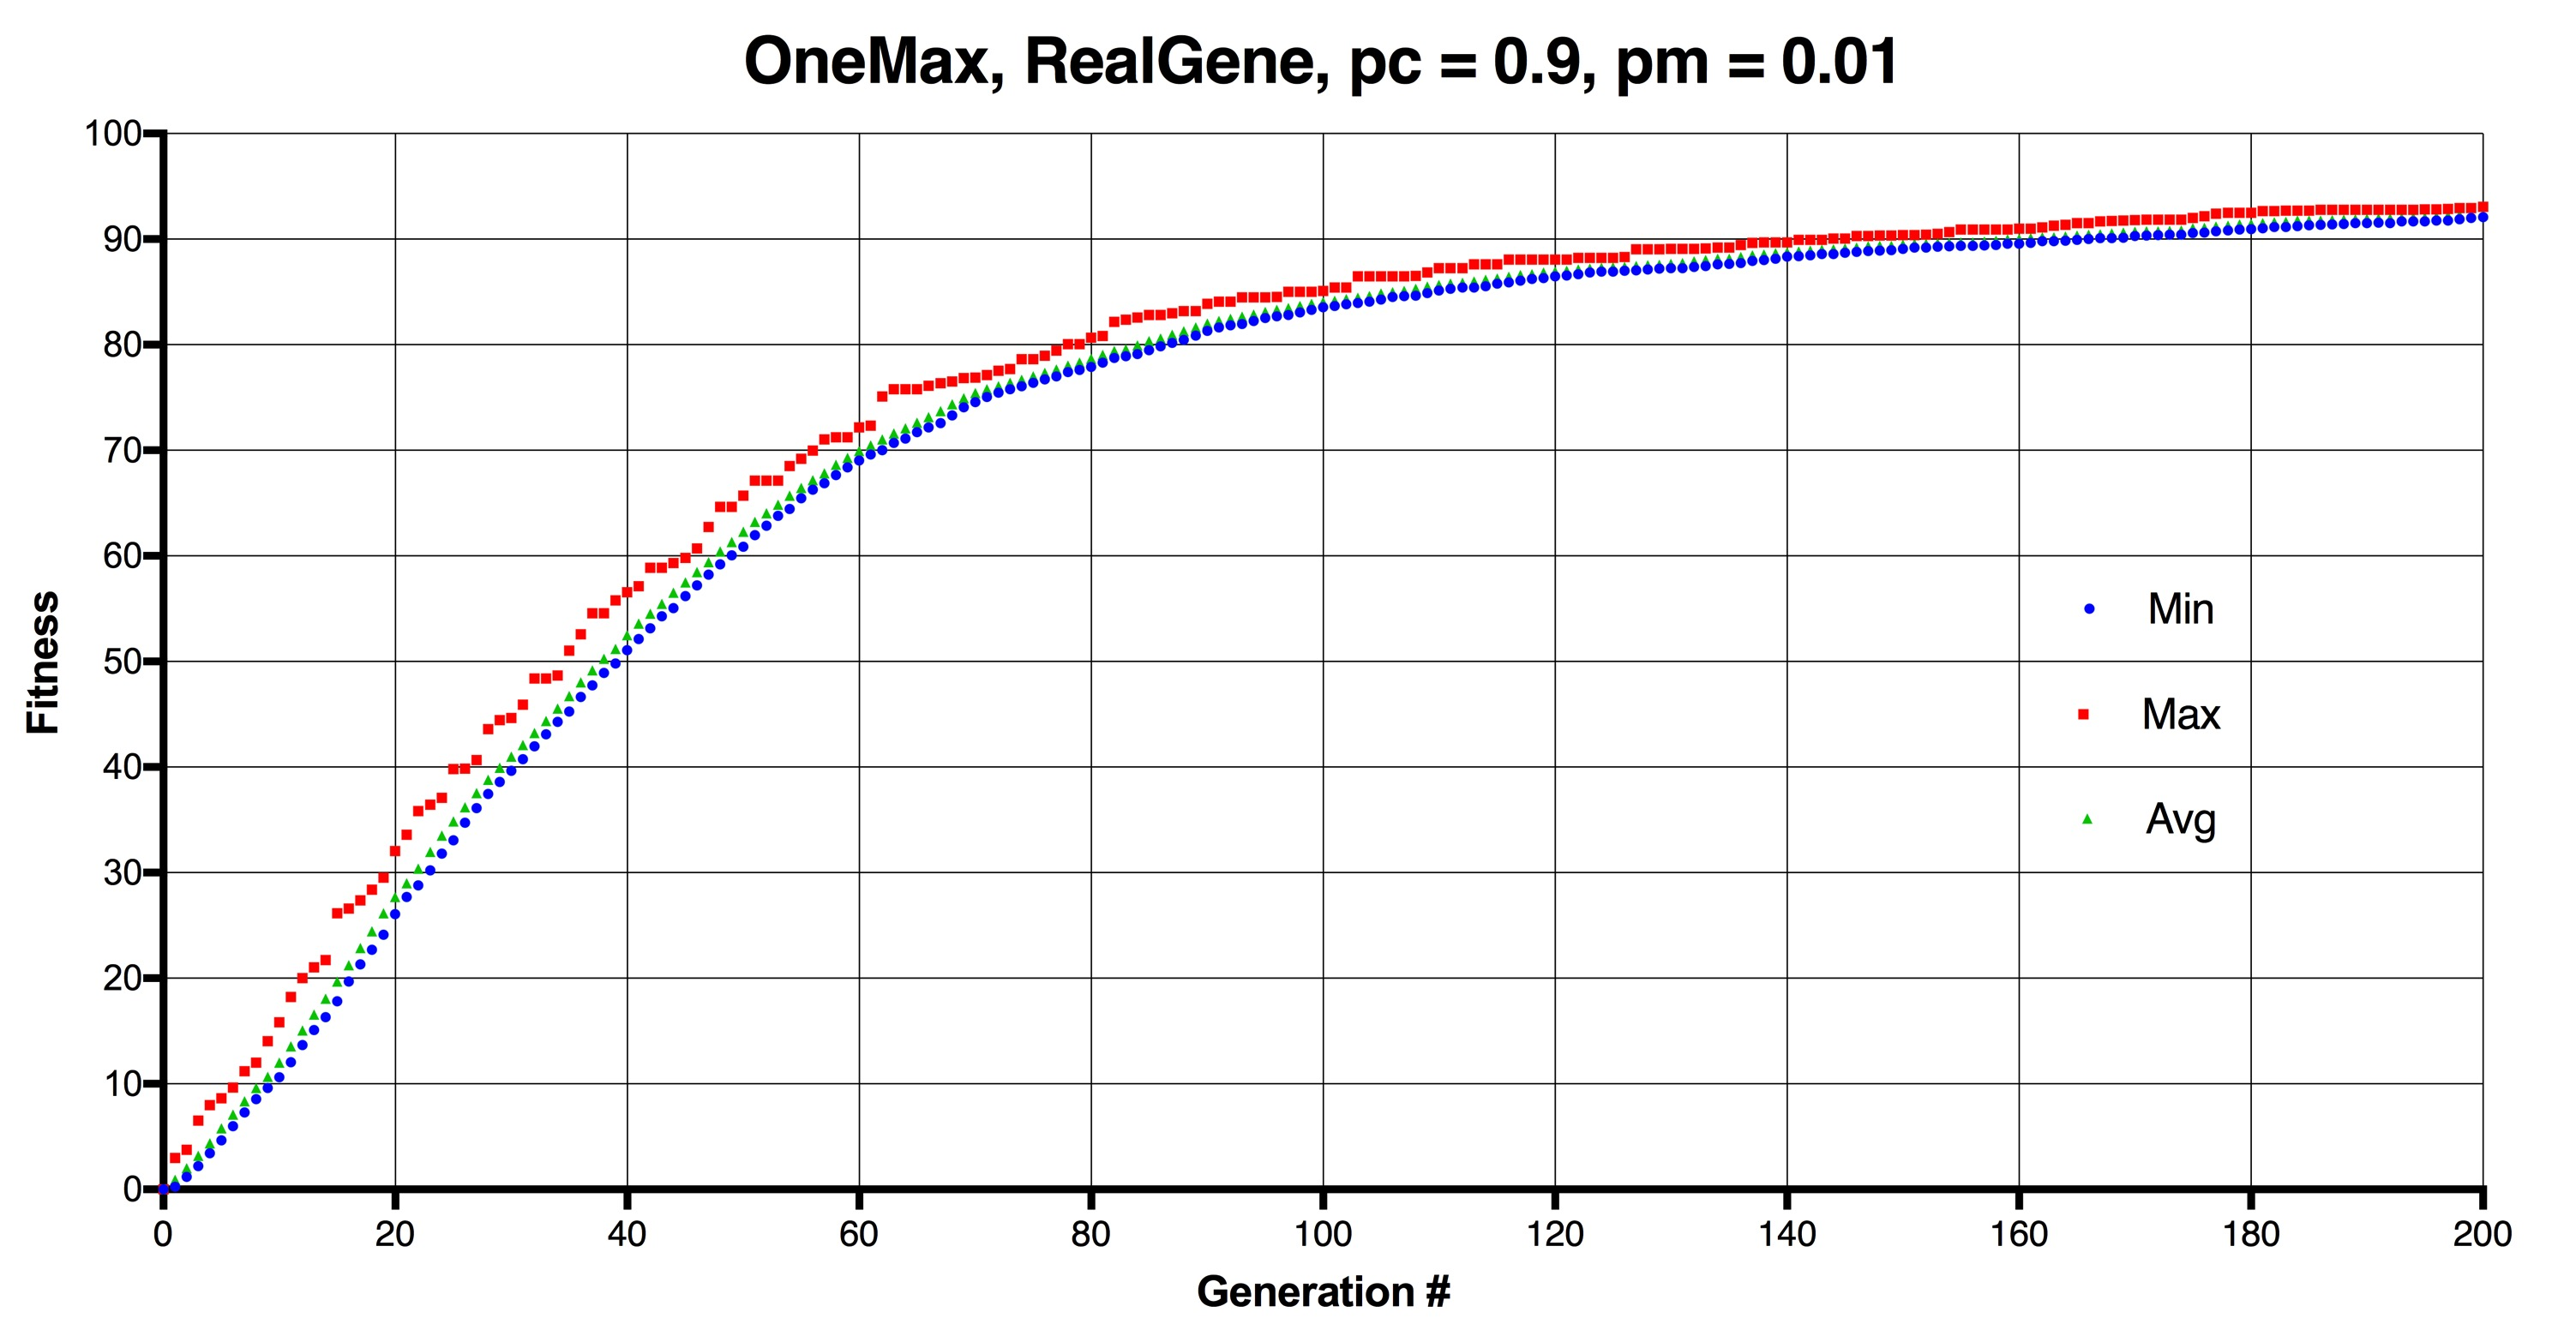
\includegraphics[width=1.0\textwidth]{onemax_real.jpg}
    \caption{Evolução do fitness para o problema do OneMax Real com mínimo, máximo e valor médio, com $p_c=0.9$ e $p_m=0.01$.}
    \label{fig:onemax_real}
\end{figure}

\begin{figure}[ht!]
    \centering 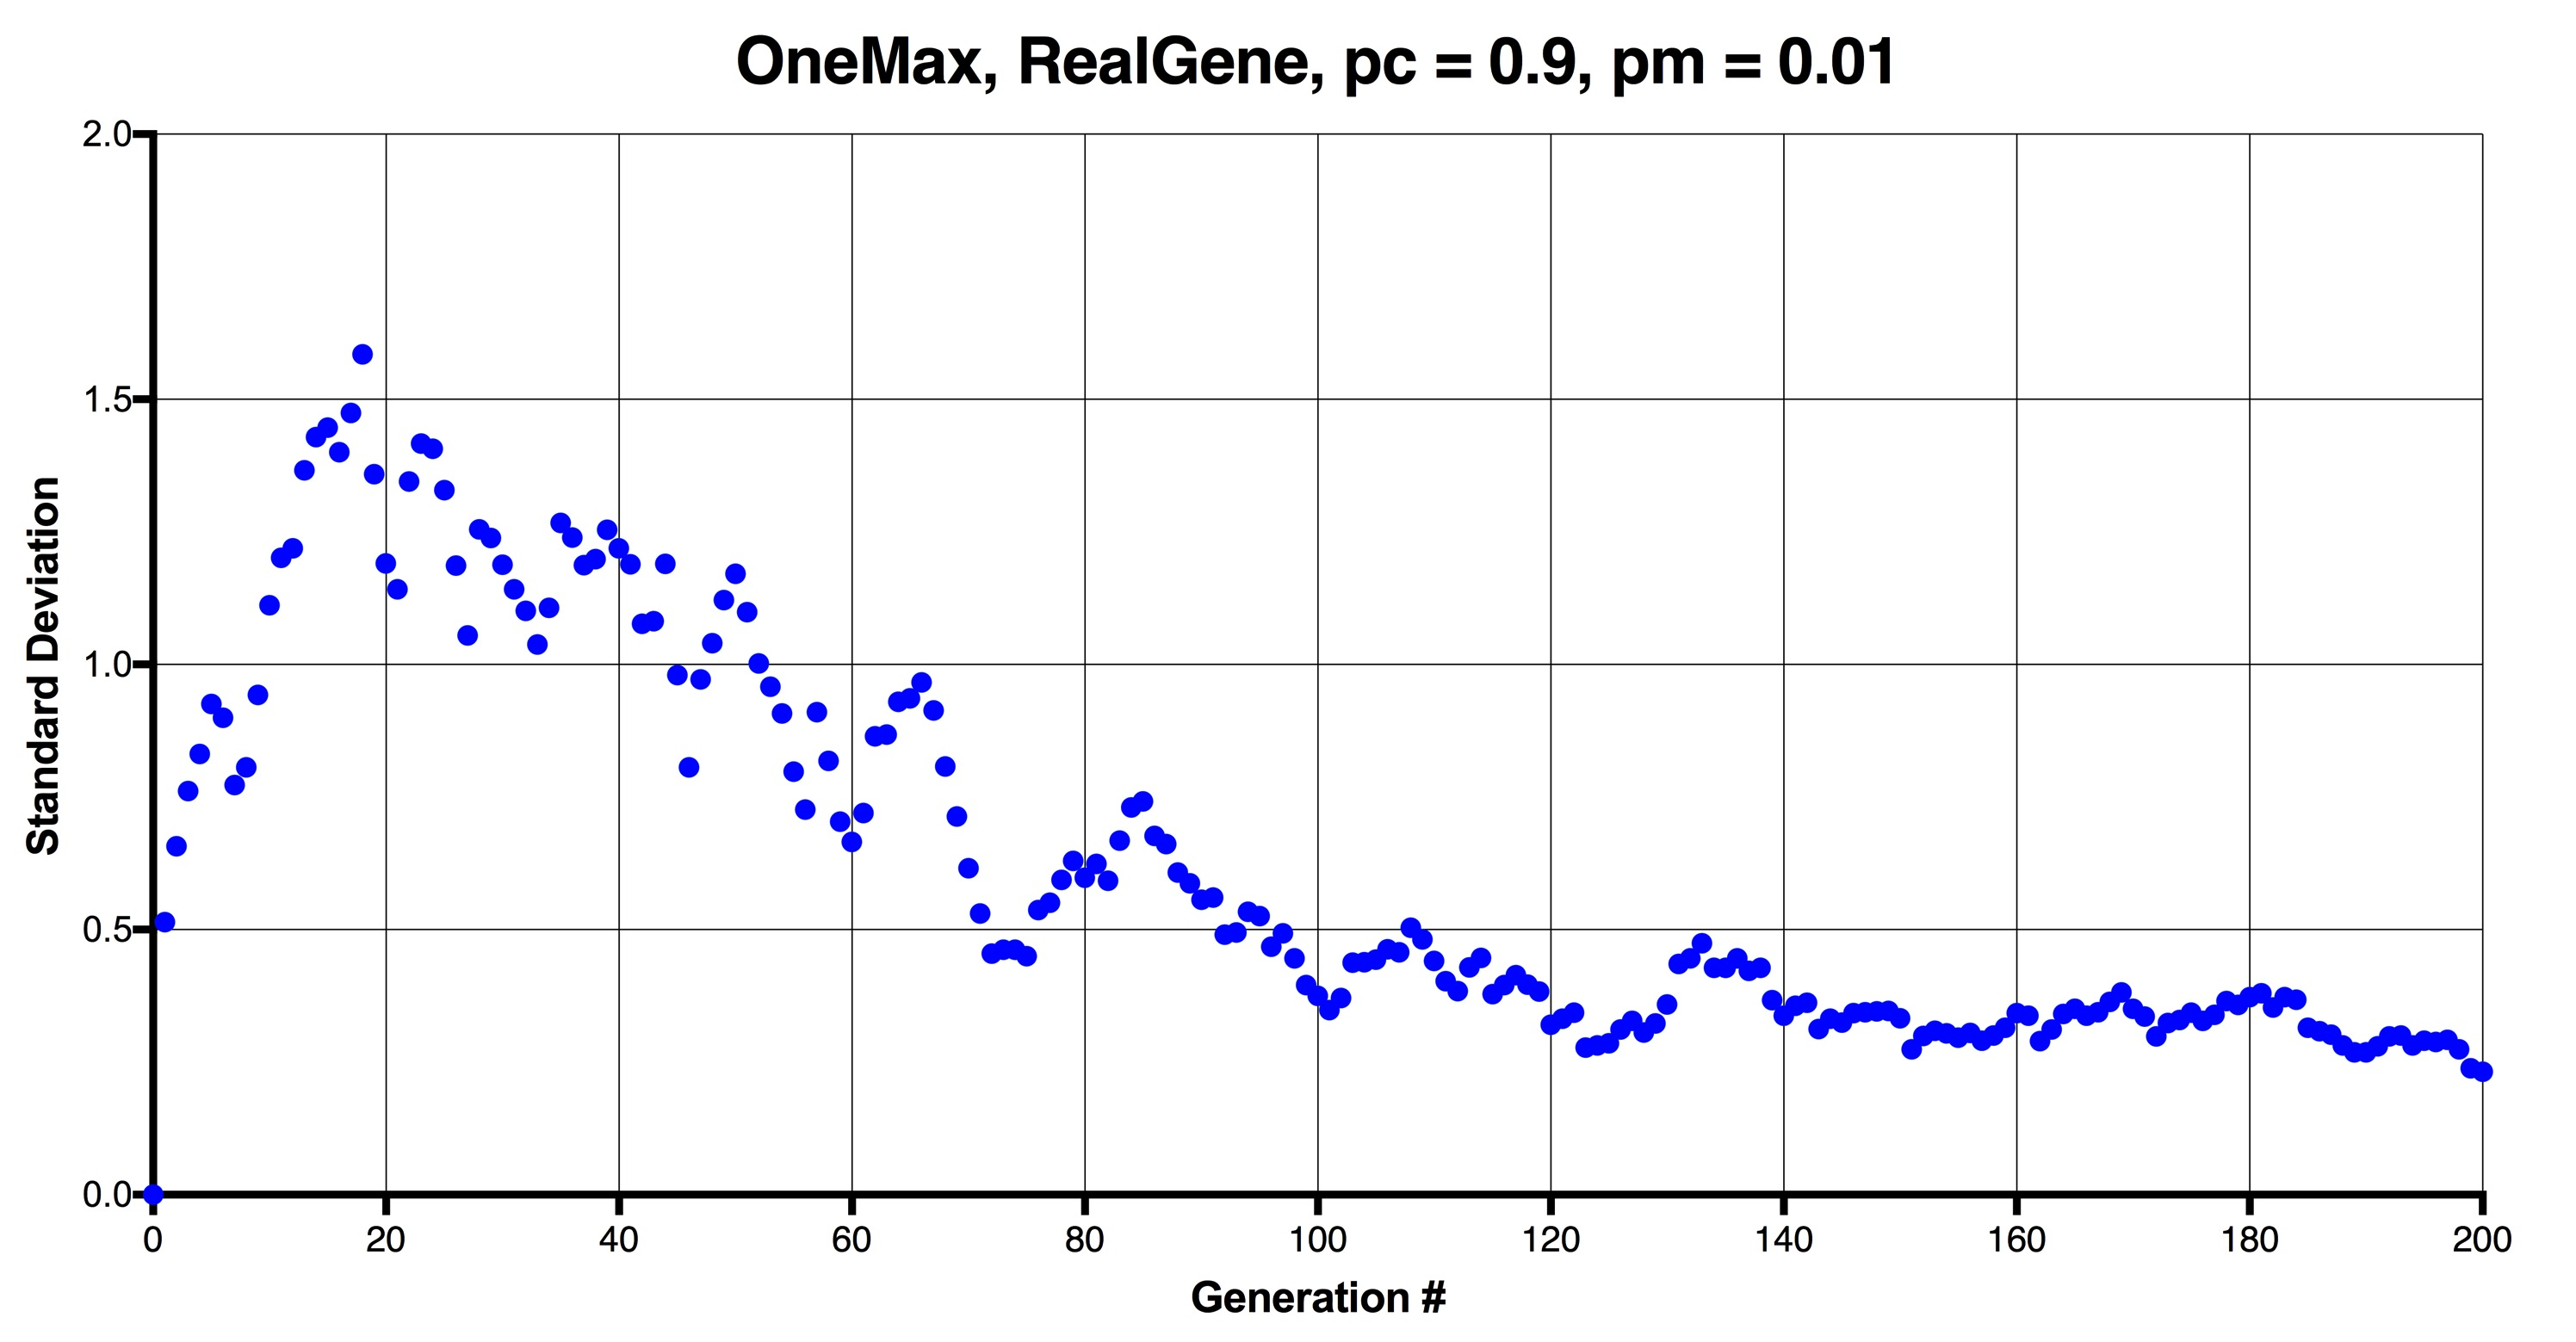
\includegraphics[width=1.0\textwidth]{onemax_real_std.jpg}
    \caption{Desvio padrão ao longo das gerações para o problema do OneMax Real, com $p_c=0.9$ e $p_m=0.01$.}
    \label{fig:onemax_real_std}
\end{figure}

Os pontos de qualquer uma das medições (média, mínimo e máximo) parecem formar uma curva. Descobri-la fugiu do escopo deste trabalho, mas tal formato pode estar associado à probabilidade de se aumentar a expressividade de um gene. Na execução deste AG, cada gene é levado para mutação com probabilidade $p_m$. Se um gene tiver uma expressividade $0 < x < 1$, a mutação (assumida uniforme) possui uma probabilidade $x$ de diminuir este valor. Logo, a expressividade aumentará (frente a uma mutação) com probabilidade:

\begin{equation}
	1 - p_mx
\end{equation}

\subsection{Caso Adaptativo}



\section{Caixeiro Viajante Adaptado}

Texto.

\begin{lstlisting}[float, floatplacement=H, caption={Mapa de cidades para o problema do Caixeiro Viajante Adaptado.}, label=lst:cidades]
[0, 633, 257, 91, 412, 150, 80, 134, 259, 505, 353, 324, 70, 211, 268, 246, 121],
[633, 0, 390, 661, 227, 488, 572, 530, 555, 289, 282, 638, 567, 466, 420, 745, 518],
[257, 390, 0, 228, 169, 112, 196, 154, 372, 262, 110, 437, 191, 74, 53, 472, 142],
[91, 661, 228, 0, 383, 120, 77, 105, 175, 476, 324, 240, 27, 182, 239, 237, 84],
[412, 227, 169, 383, 0, 267, 351, 309, 338, 196, 61, 421, 346, 243, 199, 528, 297],
[150, 488, 112, 120, 267, 0, 63, 34, 264, 360, 208, 329, 83, 105, 123, 364, 35],
[80, 572, 196, 77, 351, 63, 0, 29, 232, 444, 292, 297, 47, 150, 207, 332, 29],
[134, 530, 154, 105, 309, 34, 29, 0, 249, 402, 250, 314, 68, 108, 165, 349, 36],
[259, 555, 372, 175, 338, 264, 232, 249, 0, 495, 352, 95, 189, 326, 383, 202, 236],
[505, 289, 262, 476, 196, 360, 444, 402, 495, 0, 154, 578, 439, 336, 240, 685, 390],
[353, 282, 110, 324, 61, 208, 292, 250, 352, 154, 0, 435, 287, 184, 140, 542, 238],
[324, 638, 437, 240, 421, 329, 297, 314, 95, 578, 435, 0, 254, 391, 448, 157, 301],
[70, 567, 191, 27, 346, 83, 47, 68, 189, 439, 287, 254, 0, 145, 202, 289, 55],
[211, 466, 74, 182, 243, 105, 150, 108, 326, 336, 184, 391, 145, 0, 57, 426, 96],
[268, 420, 53, 239, 199, 123, 207, 165, 383, 240, 140, 448, 202, 57, 0, 483, 153],
[246, 745, 472, 237, 528, 364, 332, 349, 202, 685, 542, 157, 289, 426, 483, 0, 336],
[121, 518, 142, 84, 297, 35, 29, 36, 236, 390, 238, 301, 55, 96, 153, 336, 0]
\end{lstlisting}